
\documentclass[14pt,a4paper]{extarticle}

\usepackage{fontspec}
\setmainfont{Times New Roman}
\usepackage{geometry}
\geometry{left=30mm,right=15mm,top=20mm,bottom=20mm}
\usepackage{setspace}
\onehalfspacing
\usepackage{indentfirst}
\setlength{\parindent}{1.25cm}
\usepackage{ragged2e}
\justifying
\sloppy
\usepackage{array}
\usepackage{longtable}
\usepackage{booktabs}
\usepackage{multirow}
\usepackage{enumitem}
\usepackage{etoolbox}
\usepackage{amsmath}
\usepackage{graphicx}
\graphicspath{{figures/}}
\usepackage{caption}
\usepackage{float}
\usepackage{hyperref}
\usepackage{fancyhdr}
\usepackage{titlesec}
\usepackage{tocloft}
\usepackage{xcolor}
\usepackage{listings}

\lstdefinestyle{protocol}{
  basicstyle=\ttfamily\footnotesize,
  columns=fullflexible,
  keepspaces=true,
  showstringspaces=false,
  breaklines=true,
  breakatwhitespace=true,
  frame=single,
  framerule=0.4pt,
  rulecolor=\color{black!55},
  backgroundcolor=\color{black!3},
  xleftmargin=0.15cm,
  xrightmargin=0.15cm,
  aboveskip=0.30cm,
  belowskip=0.35cm
}

\hypersetup{colorlinks=true, linkcolor=black, urlcolor=black, citecolor=black}
\pagestyle{fancy}
\fancyhf{}
\fancyfoot[C]{\thepage}
\renewcommand{\headrulewidth}{0pt}
\setcounter{tocdepth}{2}
\renewcommand{\contentsname}{Contents}
\renewcommand{\cfttoctitlefont}{\hfill\normalfont\bfseries\fontsize{14pt}{16pt}\selectfont}
\renewcommand{\cftaftertoctitle}{\hfill\par\vspace{0.55cm}}
\setlength{\cftbeforesecskip}{0.38em}
\setlength{\cftbeforesubsecskip}{0.10em}
\setlength{\cftsecindent}{0pt}
\setlength{\cftsubsecindent}{1.15cm}
\renewcommand{\cftsecfont}{\bfseries}
\renewcommand{\cftsecpagefont}{\bfseries}
\renewcommand{\cftsecleader}{\cftdotfill{2.8}}
\renewcommand{\cftsubsecleader}{\hfill}

\titleformat{\section}{\normalfont\bfseries\centering\fontsize{14pt}{16pt}\selectfont}{\thesection.}{0.65em}{}
\titleformat{\subsection}{\normalfont\bfseries\fontsize{14pt}{16pt}\selectfont}{\thesubsection.}{0.65em}{}
\titleformat{\subsubsection}{\normalfont\bfseries\fontsize{14pt}{16pt}\selectfont}{\thesubsubsection.}{0.65em}{}
\titlespacing*{\section}{0pt}{0.95cm}{0.45cm}
\titlespacing*{\subsection}{0pt}{0.50cm}{0.22cm}
\titlespacing*{\subsubsection}{0pt}{0.35cm}{0.16cm}
\captionsetup[figure]{name=Figure,labelsep=endash,font=normalsize,justification=centering}
\captionsetup[table]{name=Table,labelsep=endash,font=normalsize,justification=raggedright,singlelinecheck=false,skip=0.25cm}
\setlist[itemize]{leftmargin=1.5cm,itemsep=0.2em,topsep=0.2em}
\setlist[enumerate]{leftmargin=1.5cm,itemsep=0.2em,topsep=0.2em}
\setlength{\tabcolsep}{4.5pt}
\AtBeginEnvironment{tabular}{\small\renewcommand{\arraystretch}{1.16}}
\AtBeginEnvironment{longtable}{\small\renewcommand{\arraystretch}{1.16}}
\newcommand{\code}[1]{\texttt{#1}}
\newcommand{\frontmattertitle}[1]{%
  \begin{center}
  {\normalfont\bfseries\fontsize{14pt}{16pt}\selectfont #1}
  \end{center}
  \vspace{0.35cm}
}

\begin{document}


\begin{titlepage}
\thispagestyle{empty}
\begin{spacing}{1.0}
\vspace*{0.85cm}
\begin{center}
Federal State Autonomous Educational Institution of Higher Education\\
\textbf{\fontsize{17pt}{19pt}\selectfont Moscow Institute of Physics and Technology}\\[0.12cm]
\textbf{\fontsize{16pt}{18pt}\selectfont National Research University}\\[1.45cm]
{\small\textit{Phystech School of Applied Mathematics and Informatics}}\\
{\small\textit{Field of study: Applied Mathematics and Informatics}}\\[0.35cm]
\end{center}


\vspace{1.45cm}
\begin{center}
{\bfseries\fontsize{16.5pt}{16.5pt}\selectfont CONTEXT-CONDITIONED FiLM FOR\\
BITCOIN MARKET REGIME CLASSIFICATION}\\[0.08cm]
(Bachelor thesis)
\end{center}

\vspace{1.0cm}
\begin{flushright}
\begin{minipage}{0.56\textwidth}
{\fontsize{12.5pt}{14pt}\selectfont\textbf{Student: Jeong Jaehyeon}}\\[0.16cm]
\rule{\textwidth}{0.4pt}\\[-0.05cm]
{\small\textit{student's signature}}\\[0.30cm]

{\fontsize{12.5pt}{14pt}\selectfont\textbf{Scientific supervisor: Jin Seungmin}}\\[0.16cm]
\rule{\textwidth}{0.4pt}\\[-0.05cm]
{\small\textit{scientific supervisor's signature}}\\[0.30cm]
\end{minipage}
\end{flushright}

\vfill
\begin{center}
Moscow 2026
\end{center}
\end{spacing}
\end{titlepage}


\setcounter{page}{2}

\frontmattertitle{Abstract}
\addcontentsline{toc}{section}{Abstract}
\begingroup
\setlength{\parindent}{0pt}
\begin{spacing}{1.5}
This thesis studies whether image-based return prediction can be transferred from stock price charts to Bitcoin and whether market context can improve or explain the resulting predictions. First, a Re-image-style CNN pipeline is adapted to BTC chart images and screened across 5-, 20-, and 60-day image windows and forward-return horizons. The most stable setting is then used as the basis for context-conditioned Feature-wise Linear Modulation. In this framework, market sentiment, financial news sentiment, and derivatives/leverage variables are converted into numerical context vectors and used to generate bounded channel-wise corrections to a frozen visual CNN. The goal is predictive improvement and diagnostic interpretability. Empirically, the strongest chart-only model is difficult to outperform: OHLCV images already encode substantial technical information. Chart-derived context is mostly redundant; Fear and Greed sentiment, FinBERT news sentiment, and funding plus CFTC open-interest context provide small but interpretable gains in selected settings. Grad-CAM, correction/regression counts, and FiLM gamma/beta summaries show that the context branch acts mainly as conservative probability calibration rather than as a replacement for the visual model.

\vspace{0.35cm}
\noindent\textbf{Keywords:} Bitcoin prediction, price chart images, convolutional neural networks, Feature-wise Linear Modulation, market regime classification, FinBERT, Fear and Greed index, derivatives context, interpretability.
\end{spacing}
\endgroup

\clearpage

\begingroup
\setlength{\parindent}{0pt}
\begin{spacing}{1.5}
\tableofcontents
\end{spacing}
\endgroup

\clearpage

\frontmattertitle{List of Abbreviations}
\addcontentsline{toc}{section}{List of Abbreviations}
\noindent The following abbreviations are used throughout the thesis. Terms that appear only in tables or implementation notes are included when they are necessary for interpreting the experimental results.

\vspace{0.25cm}
\begin{center}
\begin{longtable}{>{\bfseries}p{0.24\textwidth}p{0.62\textwidth}}
\toprule
\textbf{Abbreviation} & \textbf{Meaning}\\
\midrule
\endfirsthead
\toprule
\textbf{Abbreviation} & \textbf{Meaning}\\
\midrule
\endhead
AP & Average Precision\\
BB & Bollinger Bands\\
BTC & Bitcoin\\
CFTC & Commodity Futures Trading Commission\\
CNN & Convolutional Neural Network\\
F\&G & Fear and Greed Index\\
FiLM & Feature-wise Linear Modulation\\
FSI & Financial Stress Index\\
Grad-CAM & Gradient-weighted Class Activation Mapping\\
MA & Moving Average\\
MFI & Money Flow Index\\
OHLC & Open, High, Low, Close\\
OHLCV & Open, High, Low, Close, Volume\\
OI & Open Interest\\
ROC-AUC & Receiver Operating Characteristic Area Under the Curve\\
RORO & Risk-on / Risk-off\\
RV & Realized Volatility\\
SVD & Singular Value Decomposition\\
VB & Volume Bars\\
\bottomrule
\end{longtable}
\end{center}

% The abbreviations table belongs to the front matter and should not
% advance the numbering of thesis result tables.
\setcounter{table}{0}

\clearpage

\section{Introduction}

\subsection{From visual price patterns to market regimes}

A long tradition in financial prediction asks whether past prices contain information about future returns. Classical technical analysis answers this question by designing explicit patterns or indicators: moving averages, reversals, momentum, volatility bands, and volume confirmation. The image-based approach changes the question. Instead of specifying a small set of patterns in advance, it represents recent market history as a chart and lets a convolutional neural network learn the visual configurations that are most predictive of the target.

This thesis applies the chart-imaging perspective of Jiang, Kelly, and Xiu to Bitcoin market regime classification [1]. The empirical label is the sign of the 20-day forward BTC return, so the task can also be read as 20-day direction prediction. The visual input is a 60-day chart image. Depending on the specification, the chart can contain OHLC bars, a moving-average line, and volume bars. This representation is attractive because it lets the model learn price, trend, volatility, and volume patterns directly from visual structure rather than from a manually selected indicator list.

At the same time, Bitcoin is not only a price chart. It trades continuously, reacts to news and sentiment, and is strongly affected by derivatives activity and leverage conditions. The same visual pattern can therefore have different implications in different regimes. A weak recovery may be interpreted differently when market sentiment is improving, when news flow is negative, or when funding and open interest suggest crowded leverage. The central question of this thesis is whether such external context can condition the interpretation of visual chart features.

The empirical challenge is that the visual model is already strong. The strongest chart-only BTC baseline in this work uses 60-day OHLC images with moving-average and volume information and reaches an accuracy mean of 0.579320 and ROC-AUC mean of 0.584862 across five seeds. A context model must therefore be compared against this strong baseline, not against an artificially weak reference.

\subsection{Research design}

The object of research is Bitcoin market regime classification from price-chart images, where the regime label is represented by the 20-day return direction. The subject of research is context-conditioned modulation of a chart-image convolutional neural network by market sentiment, derivatives/leverage features, and news-derived signals.

The aim of the work is to evaluate whether context-conditioned Feature-wise Linear Modulation can improve or explain the predictions of a strong BTC chart-image classifier [2]. The design follows two principles. First, the visual baseline is selected before context is added. This selection is not fixed to the 20-day horizon at the beginning. The BTC chart-only stage first screens 5-, 20-, and 60-day image windows together with 5-, 20-, and 60-day forward-return horizons. Only configurations that show a defensible signal in this BTC screening are advanced to the more expensive five-seed robustness check. The strongest and most stable family is then used as the baseline for context experiments. Second, the final FiLM protocol freezes the trained visual CNN and classifier, so the context branch can only make small bounded corrections to the final feature representation.

This distinction is important for the interpretation of the thesis. The original Re-Imagining Price Trends stock-market pipeline provides the methodological reference, but it is not used as a mechanical cutoff rule for BTC model selection. In the BTC experiments, weak configurations are filtered mainly by their own BTC validation and test behavior, especially accuracy relative to the majority-class baseline and ROC-AUC. The selected five-seed check confirms that the $I60/R20$ family survives seed variation, while the tested $I20/R20$ family falls below the majority-class baseline on average. Therefore, the later 20-day regime experiments are the result of screening and robustness checking, not an a priori assumption that the 20-day horizon must be best.

The research objectives are:
\begin{enumerate}
\item build and validate a reproducible chart-image prediction pipeline for BTC OHLCV data;
\item screen short-, medium-, and long-horizon chart-only BTC baselines and select a robust visual configuration for the final context experiments;
\item construct context vectors from technical indicators, market sentiment, derivatives/leverage variables, macro stress proxies, news embeddings, and financial sentiment;
\item implement FiLM-based conditioning where the context vector generates channel-wise scale and shift parameters;
\item compare standard fusion models with a baseline-preserving protocol where the visual CNN and classifier are frozen;
\item evaluate global metrics and conditional correction/regression behavior;
\item analyze selected predictions with Grad-CAM heatmaps and FiLM gamma/beta summaries [3].
\end{enumerate}

\subsection{Research focus and empirical questions}

The research questions follow from two limitations of standard multimodal financial prediction. First, common fusion schemes such as concatenation, gating, or generic attention can combine chart and context features, but they do not clearly show how market context changes the internal chart representation used for the regime decision. A model may improve or fail, yet the role of context remains difficult to inspect. Second, if the whole visual model is retrained together with context, it becomes unclear whether a change in prediction comes from useful context, from changed visual filters, or from optimization instability.

FiLM is used in this thesis as an explicit conditioning interface. A context vector produces feature-wise scale and shift parameters, $\gamma(c)$ and $\beta(c)$, which modulate CNN feature maps. In the experiments, the context vector is built from sources such as Fear and Greed, FinBERT news sentiment, derivatives/leverage variables, macro stress proxies, and technical indicators. This makes it possible to ask not only whether context improves accuracy, but also whether the context path systematically amplifies, suppresses, or calibrates visual chart features.

The choice of the visual baseline is treated as a preliminary design step, not as the main research question. Before adding context, the BTC chart-only pipeline is screened across image windows, return horizons, and image specifications. The strongest selected configuration is then fixed as the reference model for the context experiments. With this reference in place, the empirical part of the thesis is organized around three questions.

\textbf{RQ1.} Do external market and news context variables improve over a strong BTC chart-image baseline, or are they mostly redundant with visual price information?

\textbf{RQ2.} Does a baseline-preserving FiLM design provide a more stable and interpretable conditioning mechanism than standard fusion methods such as concatenation, gating, or unrestricted FiLM?

\textbf{RQ3.} Under which market conditions does context-FiLM correct, calibrate, or degrade chart-only predictions, and what do the corresponding Grad-CAM and $\gamma/\beta$ summaries reveal about the modulation?

The main empirical finding is cautious but clear. The best chart-only model is difficult to improve because the chart image already contains much of the technical information used by traditional indicators. Technical context constructed from OHLCV data is mostly redundant. Standard fusion and fully trainable context models do not robustly beat the visual baseline. External context is more promising: Fear and Greed, FinBERT sentiment, and derivatives/leverage features produce small same-image improvements or better probability calibration in selected settings. The FiLM analysis shows that this context effect is usually conservative rather than large: gamma and beta changes are small, and decision changes occur only for a limited subset of samples. Therefore, the thesis does not claim that FiLM discovers a strong new predictor that dominates chart images. Its more defensible contribution is to show how context can be injected through an analyzable modulation interface and how that modulation can be inspected through correction/regression analysis, Grad-CAM, and gamma/beta summaries.

\subsection{Contribution and reproducibility}

The scientific novelty of the work is the baseline-preserving use of FiLM for financial chart-image prediction. Instead of training an unrestricted multimodal network, the trained visual CNN and classifier are frozen, and external context is allowed to make only small bounded final-block corrections. This design makes the context effect more measurable and interpretable.

The author's contribution consists of adapting the chart-image pipeline to BTC data, implementing the context construction workflow, implementing FiLM-based conditioning variants, designing the frozen bounded FiLM protocol, running the multi-seed experiments, and organizing the correction/regression and interpretability analysis. The initial chart-CNN implementation is based on the public \code{Stock\_CNN} PyTorch implementation associated with the Re-Imagining Price Trends paper [18], and the FiLM layer design follows the original FiLM paper and public implementation [2,19]. BTC preprocessing, context construction, frozen-training variants, and diagnostic exports are implemented as extensions for this thesis.

The experiments are organized as code notebooks, scripts, result tables, and local bundles. Raw API keys and raw third-party news text are not stored in the public repository. Large checkpoints are treated as local or Kaggle artifacts. Derived tables and summarized results are used in the thesis text. The final repository should contain only reproducible code, summarized outputs, and documentation consistent with data licenses.

\subsection{Thesis structure}

Section 2 positions the work in relation to chart-image prediction, multimodal fusion, FiLM, and financial sentiment. Section 3 describes the construction of Bitcoin chart images and context sources. Section 4 defines the context-FiLM framework and the frozen visual protocol. Section 5 reports the empirical design and main results. Section 6 interprets the results, discusses robustness checks and limitations, and Section 7 concludes.

\clearpage

\section{Related Work and Positioning}

\subsection{Chart images in financial prediction}

Technical analysis has traditionally represented price behavior through manually designed indicators. Moving averages, oscillators, Bollinger Bands, realized volatility, and volume measures are examples of such features. They are easy to compute and interpret, but they require the researcher to decide in advance which transformations are relevant. Image-based financial prediction changes the representation. Instead of computing a small set of indicators, it renders price history as a chart and lets a convolutional neural network learn local visual structures.

The Re-image approach is the main methodological starting point for this thesis [1]. It shows that historical price information can be converted into images and used for return prediction. The contribution of this thesis is not to repeat the equity experiment directly, but to transfer the idea to Bitcoin and study whether external market context can condition a strong chart-image baseline.

A key advantage of chart images is that they can combine several visual signals. In the strongest BTC baseline used here, the chart includes OHLC bars, a moving-average line, and volume bars. The CNN therefore sees both price movement and volume confirmation. This is important because later experiments show that explicitly adding some technical indicators as context gives little improvement. The likely reason is that the visual model already observes much of the same information.

\subsection{Bitcoin forecasting and market context}

Bitcoin differs from equities in several ways. It trades continuously, has high volatility, and is strongly influenced by sentiment, liquidity, derivatives activity, and news events. Many BTC forecasting studies therefore combine price features with alternative data. Sentiment indexes, social-media measures, on-chain activity, funding rates, open interest, and macro stress indicators are common candidates.

The difficulty is that context features can be noisy. A news headline may be semantically related to Bitcoin but not predictive of the next 20-day return. A macro stress index may move slowly relative to the target horizon. A technical indicator may duplicate information already visible in the chart. For this reason, context must be evaluated against a strong chart-only baseline under the same split and horizon.

\subsection{Multimodal fusion}

Multimodal fusion is often implemented by concatenating visual, numerical, and textual representations before the classifier. This is simple but not always interpretable. If the model improves, it is hard to identify whether the gain came from better visual learning, a stronger classifier, or actual context conditioning. If the model fails, it is hard to determine whether the context source is uninformative or whether the fusion mechanism is unstable.

This thesis separates these effects by first selecting a strong chart-only model and then freezing it. The context branch is trained as a small modulation layer. This protocol asks a narrower but clearer question: given a trained visual predictor, can market context calibrate its final feature representation?

\subsection{Feature-wise Linear Modulation}

Feature-wise Linear Modulation applies a context-dependent affine transformation to neural features [2]. If $F$ is a feature map and $c$ is a context vector, FiLM computes
\begin{equation}
\mathrm{FiLM}(F,c)=\gamma(c)\odot F+\beta(c),
\end{equation}
where $\gamma(c)$ and $\beta(c)$ are generated by a conditioning network. In visual reasoning, the context is often a natural-language question. In this work, the prediction question is fixed, and the variable input is market context. A small MLP is therefore sufficient to generate $\gamma$ and $\beta$.

FiLM is suitable for this thesis because it offers a structured path for interpretation. When context changes a prediction, gamma and beta describe how strongly the final visual channels were scaled or shifted. This does not make the model causal, but it is more informative than a single hidden vector produced by unrestricted concatenation.

\subsection{News embeddings and financial sentiment}

News can be represented in several ways. Recent financial work has used large language models and text representations to extract signals from news and other textual information [4,5]. A generic embedding model maps text into dense vectors that preserve semantic similarity [6]. This is useful for comparing or clustering headlines, but it does not necessarily extract directional market sentiment. A financial sentiment model such as FinBERT, built on the BERT architecture and adapted to financial sentiment, is more directly aligned with positive, neutral, and negative financial tone [7,8,9].

This distinction is visible in the experiments. Generic headline embeddings are close to the baseline but do not provide a clear hard-accuracy improvement. FinBERT sentiment improves ranking and calibration, and FinBERT combined with Fear and Greed gives the best news-context result. This supports the idea that news features should be aligned with the prediction problem rather than treated as generic text vectors only.

\subsection{Explainability for chart models}

The thesis uses Grad-CAM to visualize which chart regions contribute to the prediction [3]. Grad-CAM is not a proof of causal reasoning. It is a diagnostic that helps check whether the visual model attends to plausible chart areas. In this work, Grad-CAM is combined with correction/regression analysis and FiLM gamma/beta summaries. The goal is to interpret not only where the CNN looked, but also how external context changed the final probability.

\subsection{Positioning of this work}

The research gap is the interaction between a strong chart-image baseline and external context. Many studies add context to price features, and many studies use sentiment or news for financial prediction. Fewer studies ask whether a chart-image CNN should be preserved and only conditionally modulated. This thesis contributes to that question by comparing multiple context sources under a frozen bounded FiLM protocol.

\clearpage

\section{Imaging Bitcoin Market Data and Context Sources}

\subsection{Target definition and regime label}

Each sample is indexed by a date $t$. The model receives a chart image ending at that date and, when used, context features available up to the same date. Following the Re-Imagining Price Trends setup, the label is defined from the sign of a future return over a fixed horizon $h$. The screening stage considers $h \in \{5,20,60\}$ together with multiple image-window lengths. For a given horizon, the forward return is
\begin{equation}
R_h(t)=\frac{P_{t+h}}{P_t}-1,
\end{equation}
and the corresponding binary direction label is
\begin{equation}
y_t^{(h)}=\begin{cases}1,&R_h(t)>0,\\0,&R_h(t)\leq0.\end{cases}
\end{equation}
Thus the general task is BTC direction prediction at horizon $h$. In the final context-conditioned experiments, the most stable screened setting is a 60-day image window with $h=20$. This 20-day direction label is used as a practical binary market-regime label: positive future return is treated as an upward regime, and non-positive future return as a downward regime.

\subsection{Imaging market history}

Four chart-image specifications are used. The first contains only OHLC bars. The second adds a moving-average line. The third adds volume bars. The fourth combines OHLC bars, moving average, and volume bars. The BTC OHLCV source is a Binance-based historical Bitcoin dataset distributed through Kaggle [11]. All main image comparisons use a 60-day image window and a 20-day return horizon.

\begin{figure}[H]
\centering
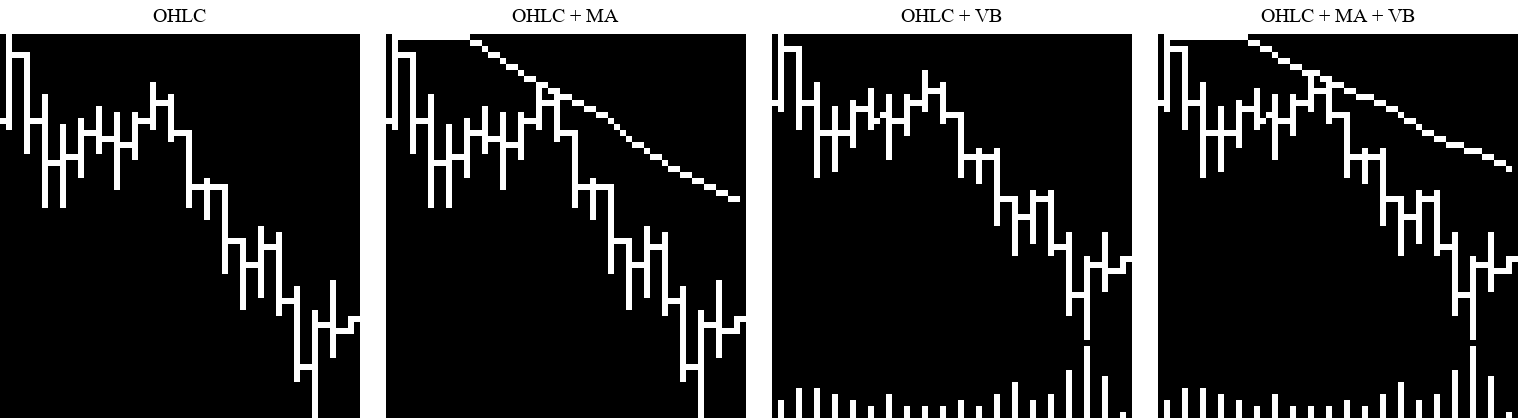
\includegraphics[width=0.95\textwidth]{chart_image_variants.png}
\caption{Chart-image encodings used by the CNN}
\end{figure}

\begin{table}[H]
\caption{Chart-image specifications used in the main experiments}
\begin{center}
\begin{tabular}{p{0.22\textwidth}p{0.56\textwidth}p{0.14\textwidth}}
\toprule
\textbf{Specification} & \textbf{Visual content} & \textbf{Role}\\
\midrule
\code{ohlc} & Open, high, low, and close bars & price-only baseline\\
\code{ohlc\_ma} & OHLC bars and moving-average line & trend-augmented baseline\\
\code{ohlc\_vb} & OHLC bars and volume bars & volume-aware baseline\\
\code{ohlc\_ma\_vb} & OHLC bars, moving average, and volume bars & strongest visual baseline\\
\bottomrule
\end{tabular}
\end{center}
\end{table}

Each image specification requires its own trained checkpoint, because the convolutional filters are tied to the visual encoding. A model trained on a volume-bar image cannot be assumed to represent the same features as a model trained on a price-only image.

\subsection{Sentiment context}

The Fear and Greed index is used as compact market sentiment context [10]. It is not directly drawn from the chart image and can therefore provide information that is external to OHLCV. The feature set includes raw values and trailing-window summaries. In the final protocol, these values are normalized on the training split and then passed to the context MLP.

\subsection{Chart-derived technical context}

Technical context includes features such as Bollinger statistics, Money Flow Index, and realized volatility. These features are useful as a test of redundancy. Since they are derived from the same OHLCV history that the image already contains, a strong CNN may already learn similar information visually. The results support this interpretation: technical context gives only very small same-image changes.

\subsection{Derivatives and leverage context}

Derivatives context is constructed separately from macro risk-on/risk-off context. It contains two feature families. The first family is based on BitMEX XBTUSD perpetual-swap data [13]. It includes funding-rate summaries over trailing windows, such as mean, sum, absolute mean, minimum, and maximum funding, together with derivatives-activity variables such as trades, volume, turnover, home notional, and foreign notional. Funding is included because perpetual-swap funding reflects the balance between leveraged long and short demand. Persistently high positive funding can indicate crowded long exposure, while negative funding can indicate short-side pressure or stress.

The second family is based on official CFTC/CME Bitcoin futures Commitment of Traders data [14]. It includes open interest and net-positioning ratios for trader groups such as leveraged money, asset managers, and dealers. These weekly variables are used as slower positioning context from the regulated futures market. To avoid lookahead, CFTC values are treated as available only after the report-release lag and are then forward-filled to daily samples. All normalization and clipping statistics are fitted on the training split only.

The final derivative feature sets are selected from this inventory after the feature audit. The two main variants are \code{funding\_only} and \code{funding\_plus\_cftc\_oi}. They are conceptually different from chart-derived technical indicators because leverage pressure and futures positioning are not directly visible in an OHLCV image. The best structured-context positive case in the thesis comes from adding funding plus CFTC open-interest context to the volume-aware chart baseline.

\subsection{Macro stress and RORO context}

Macro stress context is treated as a separate regime proxy, not as a derivatives feature. The public risk-on/risk-off proxy is inspired by the direction logic of risk-appetite indexes such as the KC Fed RORO framework, but it is not a replication of the full KC Fed proprietary input set. The proxy uses public variables oriented so that larger values correspond to stronger risk-off pressure: VIX increases, negative S\&P 500 returns, U.S. dollar strength, and negative changes in the 10-year Treasury yield. Public macro and market series are obtained from OFR, FRED, and Yahoo Finance sources where applicable [15,16,17]. These components are standardized on the training split, combined through a train-fitted first principal component, and summarized with rolling level, mean, change, and volatility features.

\subsection{News-derived context}

The news branch uses two representations. First, Bitcoin-related headlines are taken from a public Hugging Face news dataset and transformed into headline embeddings aggregated across trailing windows [12]. Second, FinBERT converts headlines into financial sentiment probabilities [8,9]. The final news-context candidate combines FinBERT sentiment aggregates with Fear and Greed context.

\subsection{No-lookahead policy}

All features are aligned chronologically. Context values must be known at or before the prediction date. Rolling windows use past values only. Publication-sensitive features are shifted where necessary. Train-only statistics are used for standardization. This is essential because even small leakage can invalidate financial prediction results. The strict chronological boundary in the final BTC experiments is the out-of-sample test split: all test samples start in 2021 or later. Inside the pre-2021 development pool, training and validation samples are randomly separated. Therefore, validation is used only for model selection and early stopping, while the thesis conclusions are based on the post-2021 test period.

\clearpage

\section{Context-FiLM Framework}

\subsection{Visual baseline CNN}

The visual model is a convolutional neural network that maps a chart image to the probability of a positive future return at a chosen horizon. The chart-only baseline is first trained without any external context. After screening multiple image-window and return-horizon combinations, the selected visual baseline is used as the reference point for the context experiments.

The strongest baseline is the $I60/R20$ model with the \code{ohlc\_ma\_vb} image specification. It is important that this model is not weak: it already combines price, trend, and volume information visually. This makes the context-conditioning task stricter and more realistic.

\subsection{Context encoder}

For each sample, the selected context variables form a vector $c_t$. A small multilayer perceptron maps $c_t$ to a hidden context representation $h_t$:
\begin{equation}
h_t=g_\theta(c_t).
\end{equation}
Depending on the ablation, this representation can be concatenated to visual features, used as a gate, or used to generate FiLM parameters.

\subsection{Bounded final-block FiLM}

The final model uses bounded FiLM on the last visual feature block. Let $F_t$ be the final convolutional feature representation. The context MLP generates raw modulation parameters, which are bounded by a hyperbolic tangent:
\begin{equation}
\gamma_t=1+s\tanh(a_t),
\end{equation}
\begin{equation}
\beta_t=s\tanh(b_t),
\end{equation}
\begin{equation}
F'_t=\gamma_t\odot F_t+\beta_t.
\end{equation}
The main scale is $s=0.02$. Thus $\gamma_t$ is restricted to the interval $[0.98,1.02]$ and $\beta_t$ to $[-0.02,0.02]$.

This restriction is not arbitrary. It follows from the experimental objective. The chart-only model is already strong, so context should not be allowed to overwrite the visual representation. Bounded FiLM treats context as calibration. If a larger or unconstrained FiLM branch is used, the context branch can destabilize the classifier and make the comparison harder to interpret.

The later scale and relaxation checks support this conservative choice. Stronger FiLM settings can move probabilities and sometimes improve ranking or calibration metrics, but they do not give a clearer hard-directional gain over the visual baseline. The final thesis model therefore keeps the small bound and treats context as a controlled correction layer rather than as a second full predictor.

\begin{figure}[H]
\centering
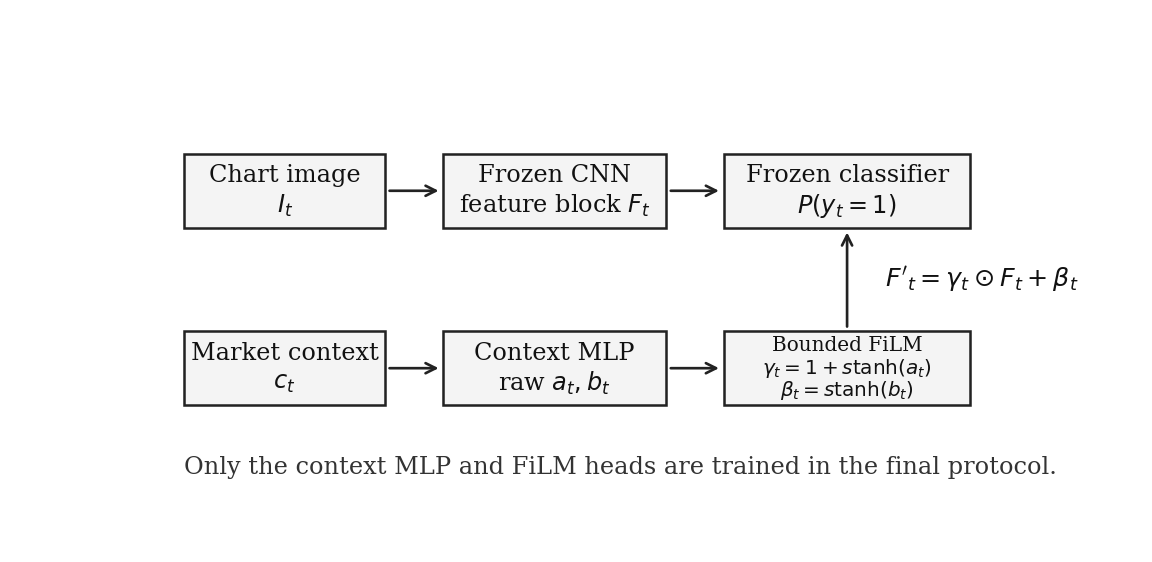
\includegraphics[width=0.92\textwidth]{bounded_film_protocol.png}
\caption{Baseline-preserving context-FiLM protocol}
\end{figure}

\subsection{Baseline-preserving frozen protocol}

The trained chart CNN and classifier are frozen in the final protocol. Only the context encoder and FiLM heads are trained. This design isolates context usefulness from changes in visual filters. It also matches the research question: can market context calibrate an already trained visual predictor?

Earlier unrestricted context models were less stable. They sometimes changed the internal visual representation in ways that reduced the strong baseline. Freezing the visual model prevents this and makes the gamma/beta values more meaningful.

\subsection{Evaluation metrics}

The three main predictive metrics are accuracy, ROC-AUC, and Brier score. Accuracy measures hard decision quality at the chosen threshold. ROC-AUC measures ranking quality independent of one threshold. Brier score measures probability calibration, that is, whether the predicted upward probability is numerically reliable. Average precision and F1 are reported as diagnostic metrics because the class distribution is not perfectly balanced. Positive-class rate and predicted-positive rate are tracked to detect degenerate models that classify almost all samples in one direction.

The original Re-Imagining Price Trends study evaluates both statistical prediction and economic usefulness: it reports classification accuracy, forecast-return correlations, and annualized Sharpe ratios for portfolios sorted by CNN forecasts. The present setting is different because BTC is a single asset rather than a stock cross-section, so cross-sectional decile portfolios cannot be copied directly. For this reason, trading-style metrics are treated as secondary diagnostics rather than as the main objective. When available, the experiment artifacts include simple long-flat and long-short annualized returns and Sharpe ratios based on the model's directional signal. These values help check whether a small accuracy difference has economic meaning, but they are not interpreted as a complete trading backtest because transaction costs, execution constraints, and overlapping horizon effects are not the focus of the thesis.

Correction/regression analysis is used to compare a context model with the chart-only baseline. A correction occurs when the baseline is wrong and the context model is correct. A regression occurs when the baseline is correct and the context model is wrong. Net correction is the difference between corrections and regressions. This is especially useful when the global accuracy gain is small, because it shows whether context adds targeted corrections or merely changes decisions at random.

\clearpage
\subsection{Interpretability protocol}

The interpretability analysis in this thesis is diagnostic rather than causal. It does not try to prove that a particular news item or sentiment value caused a Bitcoin move. Instead, it inspects how the context branch changes the decision of a fixed chart-image model. Four connected views are used: prediction transitions, context values, FiLM modulation statistics, and Grad-CAM visualizations.

First, test samples are divided into four transition groups. A correction means that the chart-only model is wrong and the context-FiLM model is correct. A regression means that the chart-only model is correct and the context-FiLM model becomes wrong. The remaining samples are both-correct or both-wrong. This view is useful because a small aggregate accuracy change can hide where context helps and where it harms.

Second, selected correction and regression samples are inspected together with their context values. For each selected sample, the analysis reports the true direction, both model predictions, both upward probabilities, and the probability change. The same table reports Fear and Greed values, rolling sentiment statistics, FinBERT positive/neutral/negative ratios, and recent news counts. This makes it possible to interpret a probability shift against the market-context regime rather than as an isolated model output.

Third, FiLM modulation is summarized through $\Delta\gamma=\gamma-1$ and $\beta$. The mean values indicate the average signed direction of modulation, while the L2 norms measure its overall magnitude. A positive $\Delta\gamma$ increases the scale of a visual feature channel, while a negative $\Delta\gamma$ decreases it. A positive or negative $\beta$ shifts the corresponding activation upward or downward. These values are not treated as named economic features, because CNN channels do not have direct semantic labels. They only show that the context branch changed the frozen visual representation in a bounded and measurable way.

Finally, Grad-CAM compares chart-only and context-conditioned saliency maps on selected transition samples. It is not causal; it only indicates which chart regions are salient for the model output. A sample-level interpretation is accepted only when the context regime, probability shift, bounded $\gamma/\beta$ modulation, and Grad-CAM change are mutually consistent.

\clearpage

\section{Empirical Design and Results}

\subsection{Empirical questions}

The empirical evaluation is organized around the research questions. First, chart-only BTC baselines are screened across image windows, return horizons, and image specifications. For every horizon, a positive forward return defines the upward class and a non-positive forward return defines the downward class. Second, the strongest visual configurations are evaluated more robustly across multiple seeds. Third, structured context, news context, and sentiment context are tested on the selected visual baselines. Finally, conditional analysis is used to understand whether small global gains hide larger effects in specific regimes.

The principal context experiments focus on the selected $I60/R20$ setting, because this family is the most stable in the chart-only screening. In that setup, the test set contains 1,441 samples per seed and the majority-class accuracy is 0.541291. Results that are central to the thesis are reported as five-seed means, while additional screening results are used to justify which configurations deserve the full five-seed evaluation. The final split uses a pre-2021 development pool and a post-2021 out-of-sample test period. Within the development pool, the implementation randomly assigns samples to training and validation; after the image-window and label-horizon restrictions this gives 671 training samples and 287 validation samples, with date ranges 2018-04-29 to 2020-12-10 and 2018-04-30 to 2020-12-11, respectively. The test samples are chronologically held out from 2021-01-01 to 2024-12-11; for the 20-day forward-return label, the corresponding test label end dates run from 2021-01-21 to 2024-12-31. This intentionally makes the test period longer than the training period, so that the final reported results reflect a long out-of-sample regime rather than a short holdout.


\subsection{Model variants}

The evaluation follows a sequence designed to avoid misleading comparisons. The first step is always the chart-only baseline. A context model is considered useful only if it improves the same visual baseline or provides a clear conditional interpretation. This is necessary because a context model trained with a weaker image could appear useful only because the image baseline is weak, while a context model trained with a different split could appear useful because the evaluation set changed.

The tested model families are summarized in Table 2. The early fusion variants are included to establish whether simple multimodal fusion is sufficient. The frozen bounded FiLM variants are the main thesis models because they preserve the visual representation and isolate the marginal effect of context.

\begin{table}[H]
\caption{Model families evaluated in the thesis}
\begin{center}
\begin{tabular}{>{\raggedright\arraybackslash}p{0.24\textwidth}>{\raggedright\arraybackslash}p{0.32\textwidth}>{\raggedright\arraybackslash}p{0.28\textwidth}}
\toprule
\textbf{Model family} & \textbf{Description} & \textbf{Purpose}\\
\midrule
Chart-only CNN & Uses only the rendered BTC chart image & establishes the visual baseline\\
Concatenation & Joins visual and context features before classification & tests simple late fusion\\
Gating & Uses context to weight visual representation & tests multiplicative control\\
Full FiLM & Generates gamma and beta from context & tests feature-wise conditioning\\
Frozen bounded FiLM & Freezes the visual CNN/classifier and trains only bounded FiLM heads & isolates conservative context calibration\\
\bottomrule
\end{tabular}
\end{center}
\end{table}

\begin{figure}[H]
\centering
\footnotesize
\setlength{\tabcolsep}{5pt}
\renewcommand{\arraystretch}{1.25}
\begin{tabular}{>{\raggedright\arraybackslash}p{0.29\textwidth}>{\raggedright\arraybackslash}p{0.30\textwidth}>{\raggedright\arraybackslash}p{0.30\textwidth}}
\toprule
\textbf{A. Chart-only baseline} &
\textbf{B. Joint context fusion} &
\textbf{C. Frozen bounded FiLM}\\
\midrule
Image $\rightarrow$ CNN $\rightarrow$ classifier &
Image $\rightarrow$ CNN feature\newline Context $\rightarrow$ MLP\newline Fusion: concat/gating/FiLM &
Image $\rightarrow$ frozen chart CNN\newline Context $\rightarrow$ bounded FiLM\newline Frozen classifier\\
\addlinespace[0.15cm]
\textit{Updated:} CNN and classifier &
\textit{Updated:} CNN, context branch, classifier &
\textit{Updated:} context branch only\\
\addlinespace[0.15cm]
\textit{Role:} visual reference model &
\textit{Role:} context effect is mixed with visual re-learning &
\textit{Role:} marginal context calibration is isolated\\
\bottomrule
\end{tabular}
\caption{Training-regime comparison}
\end{figure}

The main reported results use the frozen bounded FiLM protocol. The other variants remain important because they explain why the protocol was chosen. Scratch-trained context models were more flexible, but they did not reliably preserve the strong visual baseline. Larger FiLM scales also increased the risk that context would change the model too strongly without producing consistent improvement. The final protocol therefore trades off maximum flexibility for stability and interpretability.

\subsection{Context-source taxonomy}

The context sources are divided into five groups. The first group is chart-derived context, such as Bollinger features, MFI, and realized volatility. These variables are useful for checking whether the CNN already learns technical information from images. The second group is sentiment-regime context, represented by F\&G. The third group is derivatives and leverage context, represented by funding features and CFTC/CME Bitcoin futures open-interest information. The fourth group is macro stress and risk-on/risk-off context, represented by FSI and public RORO proxy features. The fifth group is text-derived context, including generic headline embeddings and FinBERT sentiment.

This taxonomy is central to the interpretation of the results. If chart-derived features do not help, the result does not imply that FiLM lacks value. It may mean that the information has already been absorbed by the visual baseline. If external context helps only slightly, the result suggests that BTC chart images are strong but not complete. If generic text embeddings fail while FinBERT helps, the result suggests that task-aligned text representation is more important than high-dimensional semantic representation alone.

\subsection{Decision threshold and calibration}

Accuracy is computed from hard decisions, so it depends on the probability threshold. ROC-AUC and average precision are threshold-independent ranking metrics, while Brier score measures probability calibration. This distinction matters in the news experiments. FinBERT-only improves ROC-AUC and Brier score but does not improve accuracy. The model is therefore better at ranking and calibration, but the default threshold does not always convert this into more correct hard decisions.

For this reason, the thesis does not rely on accuracy alone. A small accuracy improvement with better Brier score and positive net corrections is more credible than a single accuracy value. Conversely, a model that improves one seed but collapses the predicted positive rate in another seed is not considered stable.

\subsection{Single-seed chart screening}

Before running five-seed experiments, the BTC chart-only pipeline is screened with one seed across image windows, return horizons, and image specifications. This step is not used as final evidence. Its purpose is to avoid spending the full multi-seed budget on configurations that are already weak in the first pass. Table 3 reports the best image specification for each image-window and return-horizon pair from the seed-42 screening run. The value 0.603053 for $I60/R20$ is therefore a screening value, not the final reported five-seed mean.

The decision label is based on this internal BTC screening, not on the stock-reproduction experiment. A setting is rejected if it does not beat the majority-class baseline or if its ROC-AUC is close to random ranking. A setting is kept for a robustness check if both quantities are positive but the margin is small. A setting is selected only when it is clearly above the majority baseline and also has a strong ROC-AUC in the screening run.

\begin{table}[H]
\caption{Seed-42 chart-only screening}
\begin{center}
\small
\setlength{\tabcolsep}{3pt}
\begin{tabular}{p{0.12\textwidth}p{0.17\textwidth}p{0.13\textwidth}p{0.13\textwidth}p{0.13\textwidth}p{0.15\textwidth}}
\toprule
\textbf{Setting} & \textbf{Best image spec} & \textbf{Acc. (s42)} & \textbf{$\Delta$ majority} & \textbf{ROC-AUC} & \textbf{Decision}\\
\midrule
$I5/R5$ & \code{ohlc\_vb} & 0.524038 & -0.002060 & 0.526619 & reject\\
$I5/R20$ & \code{ohlc\_ma} & 0.521166 & -0.020125 & 0.494538 & reject\\
$I5/R60$ & \code{ohlc} & 0.518201 & -0.024982 & 0.514058 & reject\\
$I20/R5$ & \code{ohlc\_ma} & 0.522665 & -0.003434 & 0.520839 & reject\\
$I20/R20$ & \code{ohlc\_vb} & 0.545455 & 0.004164 & 0.530915 & robust check\\
$I20/R60$ & \code{ohlc\_vb} & 0.512491 & -0.030692 & 0.501565 & reject\\
$I60/R5$ & \code{ohlc\_ma} & 0.526099 & 0.000000 & 0.519181 & reject\\
$I60/R20$ & \code{ohlc\_ma\_vb} & 0.603053 & 0.061763 & 0.616950 & select\\
$I60/R60$ & \code{ohlc} & 0.543183 & 0.000000 & 0.489131 & reject\\
\bottomrule
\end{tabular}
\end{center}
\end{table}

The screening has two implications. First, the selected setting is not chosen only because it has the highest raw accuracy. It is also the only setting with a large margin over the majority-class baseline and a clearly positive ROC-AUC. Second, short-window configurations and 60-day return labels are not reliable in this dataset. The short-window models appear close to noise, while the $R60$ models can show acceptable accuracy only because the majority class is easier to predict; their ranking quality is weak. The $I20/R20$ setting is the only borderline alternative, so it is checked with five seeds together with $I60/R20$.

\subsection{Visual baseline comparison}

\begin{table}[H]
\caption{Five-seed $R20$ robustness check}
\begin{center}
\small
\setlength{\tabcolsep}{3pt}
\begin{tabular}{p{0.13\textwidth}p{0.17\textwidth}p{0.13\textwidth}p{0.13\textwidth}p{0.13\textwidth}p{0.18\textwidth}}
\toprule
\textbf{Setting} & \textbf{Image spec} & \textbf{Acc. mean} & \textbf{$\Delta$ majority} & \textbf{ROC-AUC} & \textbf{Interpretation}\\
\midrule
$I20/R20$ & \code{ohlc} & 0.505899 & -0.035392 & 0.498583 & below majority\\
$I20/R20$ & \code{ohlc\_ma} & 0.506731 & -0.034559 & 0.499313 & below majority\\
$I20/R20$ & \code{ohlc\_vb} & 0.511312 & -0.029979 & 0.503884 & below majority\\
$I20/R20$ & \code{ohlc\_ma\_vb} & 0.511728 & -0.029563 & 0.504736 & below majority\\
\addlinespace[0.08cm]
$I60/R20$ & \code{ohlc} & 0.558085 & 0.016794 & 0.560218 & price only\\
$I60/R20$ & \code{ohlc\_ma} & 0.557529 & 0.016239 & 0.564495 & trend only\\
$I60/R20$ & \code{ohlc\_vb} & 0.567384 & 0.026093 & 0.561247 & volume helps\\
$I60/R20$ & \code{ohlc\_ma\_vb} & 0.579320 & 0.038029 & 0.584862 & strongest\\
\bottomrule
\end{tabular}
\end{center}
\end{table}

\begin{figure}[H]
\centering
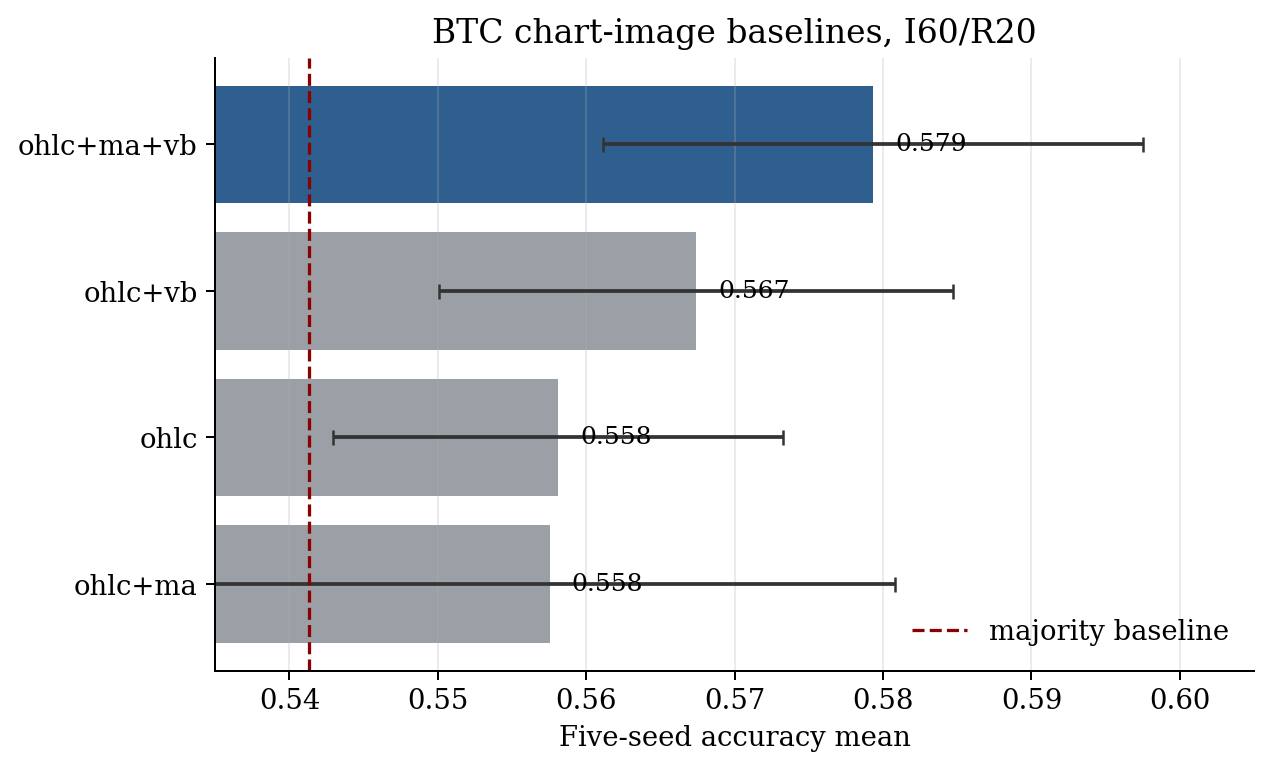
\includegraphics[width=0.88\textwidth]{visual_baseline_accuracy.png}
\caption{Five-seed accuracy of $I60/R20$ visual baselines}
\end{figure}

The five-seed robustness check changes the interpretation of the seed-42 screening number. The final reported $I60/R20$ \code{ohlc\_ma\_vb} accuracy is 0.579320, not 0.603053. The latter is only the seed-42 screening value. The $I20/R20$ family is not used as the main baseline because every five-seed variant falls below the majority-class baseline on average. The strongest robust baseline is therefore $I60/R20$ with \code{ohlc\_ma\_vb}. This result suggests that volume and trend information are useful when encoded inside the chart image. It also creates an important constraint for context experiments: chart-derived indicators must be compared against a visual model that already sees similar information.

\subsection{Technical context results}

Technical context features provide almost no same-image improvement. The accuracy changes are near zero:
\begin{equation*}
\Delta_{ohlc}=0.000000,\quad \Delta_{ohlc\_ma}=0.000139,
\end{equation*}
\begin{equation*}
\Delta_{ohlc\_vb}=0.000139,\quad \Delta_{ohlc\_ma\_vb}=0.000416.
\end{equation*}
This is a negative result, but it is informative. It indicates that many OHLCV-derived indicators are redundant with a strong visual representation. Adding them after the CNN as weak FiLM context does not reproduce the benefit of drawing the relevant information directly in the image.

\subsection{Fear and Greed context}

Fear and Greed behaves differently because it is external sentiment context. The gains remain small, but the sign is more meaningful:
\begin{table}[H]
\caption{Fear and Greed context by image specification}
\begin{center}
\small
\setlength{\tabcolsep}{3pt}
\begin{tabular}{p{0.25\textwidth}p{0.13\textwidth}p{0.13\textwidth}p{0.13\textwidth}p{0.13\textwidth}p{0.13\textwidth}}
\toprule
\textbf{Model} & \textbf{Acc.} & \textbf{$\Delta$ Acc.} & \textbf{ROC-AUC} & \textbf{$\Delta$ ROC} & \textbf{Brier}\\
\midrule
Chart-only baseline & 0.579320 & -- & 0.584862 & -- & 0.274337\\
F\&G on \code{ohlc} & 0.557668 & -0.021652 & 0.559828 & -0.025034 & 0.252753\\
F\&G on \code{ohlc\_ma} & 0.556697 & -0.022623 & 0.564479 & -0.020383 & 0.278564\\
F\&G on \code{ohlc\_vb} & 0.567939 & -0.011381 & 0.561033 & -0.023829 & 0.258102\\
F\&G on \code{ohlc\_ma\_vb} & 0.580291 & +0.000971 & 0.584930 & +0.000068 & 0.274004\\
\bottomrule
\end{tabular}
\end{center}
\end{table}

The deltas are measured against the strongest chart-only baseline, \code{ohlc\_ma\_vb}. The interpretation is cautious. F\&G does not transform the model, but it can slightly calibrate the strongest visual baseline. This supports the use of external sentiment context more than chart-derived technical context.

\subsection{Derivatives and leverage context}

The strongest same-image structured-context improvement appears with funding plus CFTC open-interest context on the \code{ohlc\_vb} baseline.
This baseline is chosen deliberately. Among the $I60/R20$ image variants, \code{ohlc\_vb} is the strongest chart-only model after \code{ohlc\_ma\_vb}. It keeps the volume-bar information that was empirically useful in the visual screening, but removes the moving-average overlay. This makes it a controlled volume-aware baseline for testing derivatives context.

This choice is important for interpretation. The moving average is a direct trend transform of the price history, so keeping it would make the comparison closer to the strongest visual model and less diagnostic. Volume bars are retained because they are not the same object as funding rates or open interest. They represent visible market activity in the chart, while funding and CFTC open interest represent leveraged futures positioning. Therefore, the experiment does not ask whether derivatives context can rescue a stripped-down price-only chart. It asks whether derivatives context adds information beyond a reasonable volume-aware chart.

This category should be separated from the macro stress and RORO experiments. CFTC open interest is used here as a futures-positioning variable, while funding is a derivatives-market leverage proxy. By contrast, FSI and RORO describe broad risk appetite and financial stress, not derivatives positioning. They were tested as macro regime controls, but they did not provide the strongest positive case and are therefore not merged into the derivative/leverage table.

\begin{table}[H]
\caption{Derivative/leverage context results}
\begin{center}
\small
\setlength{\tabcolsep}{3pt}
\begin{tabular}{p{0.25\textwidth}p{0.13\textwidth}p{0.13\textwidth}p{0.13\textwidth}p{0.13\textwidth}p{0.13\textwidth}}
\toprule
\textbf{Model} & \textbf{Acc.} & \textbf{$\Delta$ Acc.} & \textbf{ROC-AUC} & \textbf{$\Delta$ ROC} & \textbf{Brier}\\
\midrule
Chart-only baseline & 0.579320 & -- & 0.584862 & -- & 0.274337\\
OHLC+VB chart-only & 0.567384 & -0.011936 & 0.561247 & -0.023615 & 0.258306\\
Funding FiLM & 0.567661 & -0.011659 & 0.561255 & -0.023607 & 0.258085\\
Funding + CFTC OI & 0.569466 & -0.009854 & 0.561820 & -0.023042 & 0.257451\\
\bottomrule
\end{tabular}
\end{center}
\end{table}

In Table 6, both deltas are measured against the strongest chart-only baseline, \code{ohlc\_ma\_vb}. This result should not be misread. The derivative/leverage model does not beat the overall best visual baseline. Its value is instead that it improves the same \code{ohlc\_vb} image baseline by 0.002082 accuracy points. The context therefore adds information to a fixed visual representation, but it does not close the gap to the strongest chart encoding.

\subsection{News and sentiment context}

Several text representations are tested before selecting the final news-context feature. The first representation is TF-IDF followed by SVD, fitted only on the training headline windows. The second representation uses OpenAI \code{text-embedding-3-small} headline embeddings, aggregated across headlines before being reduced to a compact context vector. These representations capture lexical or semantic similarity, but they are not explicitly trained to encode financial direction. The third representation uses FinBERT sentiment probabilities, which are more directly aligned with positive, neutral, and negative financial tone. The best news-context row combines FinBERT sentiment with F\&G.

\begin{table}[H]
\caption{News and sentiment context results}
\begin{center}
\small
\setlength{\tabcolsep}{3pt}
\begin{tabular}{p{0.25\textwidth}p{0.13\textwidth}p{0.13\textwidth}p{0.13\textwidth}p{0.13\textwidth}p{0.13\textwidth}}
\toprule
\textbf{Model} & \textbf{Acc.} & \textbf{$\Delta$ Acc.} & \textbf{ROC-AUC} & \textbf{$\Delta$ ROC} & \textbf{Brier}\\
\midrule
Chart-only baseline & 0.579320 & -- & 0.584862 & -- & 0.274337\\
TF-IDF/SVD FiLM & 0.579736 & +0.000416 & 0.585353 & +0.000491 & 0.273765\\
Dense embedding FiLM & 0.578210 & -0.001110 & 0.584401 & -0.000461 & 0.273893\\
F\&G-only FiLM & 0.580291 & +0.000971 & 0.584930 & +0.000068 & 0.274004\\
FinBERT-only FiLM & 0.578487 & -0.000833 & 0.586072 & +0.001210 & 0.272739\\
FinBERT + F\&G FiLM & 0.580569 & +0.001249 & 0.585843 & +0.000981 & 0.272701\\
\bottomrule
\end{tabular}
\end{center}
\end{table}

\begin{figure}[H]
\centering
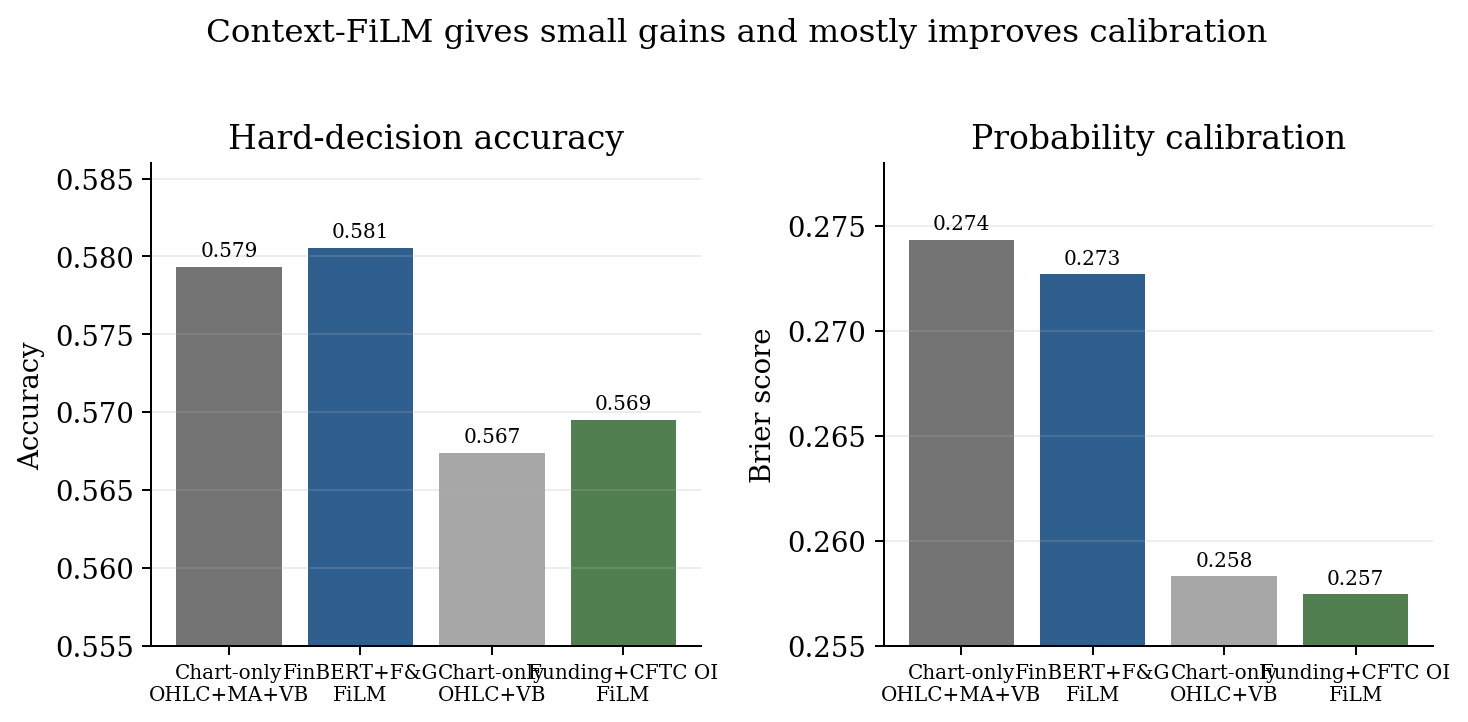
\includegraphics[width=0.96\textwidth]{context_results_accuracy_brier.png}
\caption{Summary of the strongest context cases}
\end{figure}

All rows in Table 7 use the same $I60/R20$ \code{ohlc\_ma\_vb} visual backbone. TF-IDF/SVD gives a very small positive result, while the dense embedding does not improve hard accuracy. This suggests that simply adding a high-dimensional semantic representation is not enough. FinBERT-only improves ROC-AUC and Brier score but not accuracy, which means it improves ranking and calibration more than thresholded decisions. FinBERT plus F\&G gives the best news-context accuracy among the tested news/sentiment rows. The margins are small, so the correct conclusion is not that news context dominates chart images. The correct conclusion is that sentiment-aligned text features can produce small calibration improvements more reliably than generic text representations.

\subsection{Correction and regression counts}

\begin{table}[H]
\caption{FinBERT + F\&G correction/regression by seed}
\begin{center}
\begin{tabular}{p{0.12\textwidth}p{0.15\textwidth}p{0.15\textwidth}p{0.15\textwidth}p{0.15\textwidth}p{0.14\textwidth}}
\toprule
\textbf{Seed} & \textbf{Baseline acc.} & \textbf{FiLM acc.} & \textbf{Corrections} & \textbf{Regressions} & \textbf{Net}\\
\midrule
42 & 0.603053 & 0.602359 & 9 & 10 & -1\\
43 & 0.574601 & 0.573907 & 26 & 27 & -1\\
44 & 0.562804 & 0.566967 & 34 & 28 & +6\\
45 & 0.562804 & 0.565579 & 12 & 8 & +4\\
46 & 0.593338 & 0.594032 & 14 & 13 & +1\\
Mean / sum & 0.579320 & 0.580569 & 95 & 86 & +9\\
\bottomrule
\end{tabular}
\end{center}
\end{table}

\begin{figure}[H]
\centering
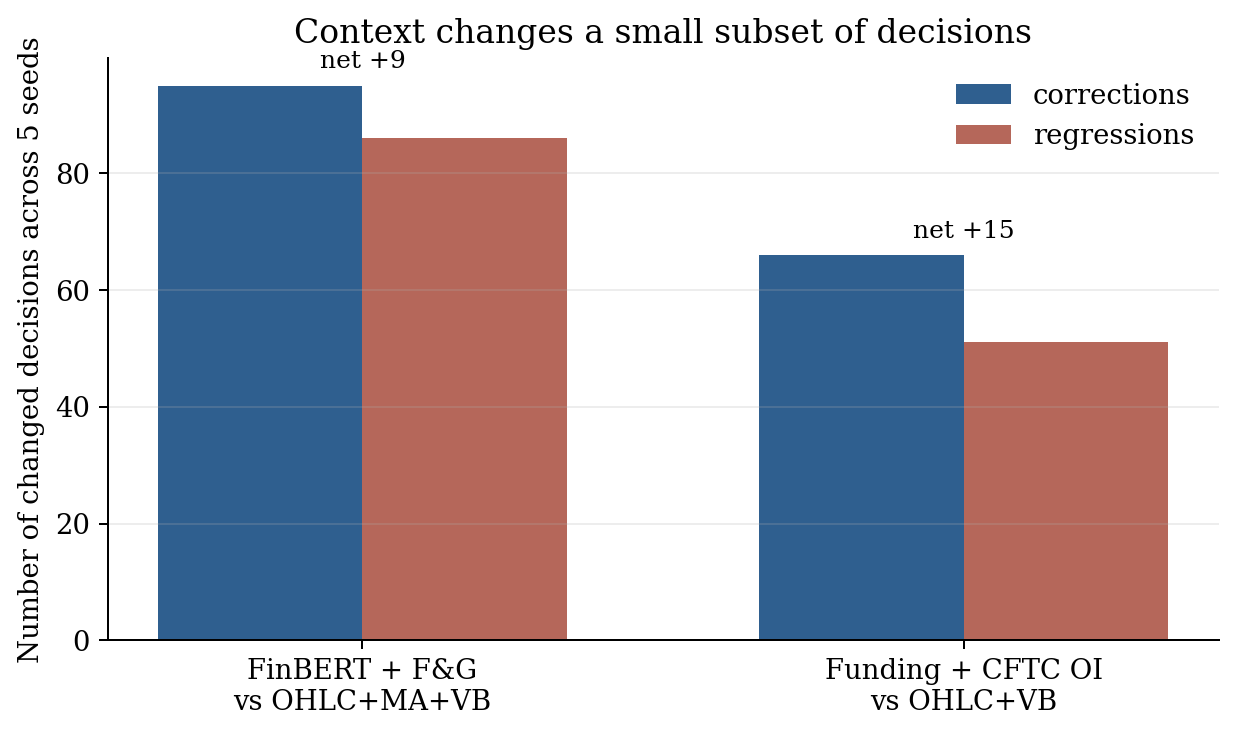
\includegraphics[width=0.86\textwidth]{correction_regression_counts.png}
\caption{Correction and regression counts}
\end{figure}

The model changes only 181 of 7,205 matched decisions, or 2.5121 percent. This confirms that bounded FiLM is conservative. Its value is not a broad replacement of the chart model but selective correction. The net correction count is also small relative to binomial noise: for the 95 corrections and 86 regressions in Table 8, a two-sided sign test gives $p\approx0.552$. Therefore, the table is interpreted as a diagnostic transition analysis rather than as a statistically significant accuracy result.

\clearpage

\section{Interpretation, Robustness, and Limitations}

\subsection{Principal findings}

The first finding is that the strongest chart image is difficult to beat. The \code{ohlc\_ma\_vb} image already includes price, trend, and volume information. As a result, adding Bollinger, MFI, or volatility features after the CNN gives little benefit.

The second finding is that external context is more defensible than chart-derived context. F\&G, FinBERT sentiment, and derivatives variables are not simply transformations of the same chart image. They can therefore add information that the CNN cannot fully infer from OHLCV visual structure.

The third finding is that the best context effects are small. The largest global accuracy improvements remain below one percentage point. This means the thesis should not claim strong multimodal dominance. The more precise claim is conditional calibration.

\subsection{Why technical context is mostly redundant}

Technical indicators are derived from price and volume history. If the chart image already contains price bars, moving average, and volume bars, then many technical variables are alternative encodings of the same information. A CNN can learn local slopes, relative price levels, bar widths, and volume bursts directly from the image. Adding those values after the CNN as a small context vector does not give the model a fundamentally new signal.

This explains why \code{ohlc\_ma\_vb} is strong and why technical FiLM does not recover the gap between weaker images and the strongest image. Some information is most useful when it is part of the visual representation itself, not when it is added later as small final-block modulation.

\subsection{Why sentiment and derivatives context can help}

F\&G, FinBERT sentiment, funding, and open interest are different. They represent market psychology, news tone, leverage, and positioning. These variables are not fully visible in the chart image. They can therefore calibrate the final prediction in conditions where the chart pattern is ambiguous.

The correction/regression evidence supports this interpretation. FinBERT+F\&G helps most in uncertain visual samples and active sentiment/news regimes. The derivatives model provides a related same-image case: funding plus CFTC open-interest context tends to lower weak bullish predictions. In both cases, context behaves as a small correction layer, not as a new dominant predictor.

The predefined N16 bucket analysis makes this derivatives result more precise. It is a conditional analysis of the controlled \code{ohlc\_vb} setting, not a replacement for the strongest \code{ohlc\_ma\_vb} visual model. The full-test same-image gain is small, but corrections concentrate where the visual model is uncertain and funding is high. Table 9 reports the predefined buckets.

\begin{table}[H]
\caption{Conditional derivatives/leverage buckets}
\begin{center}
\small
\setlength{\tabcolsep}{3pt}
\begin{tabular}{p{0.34\textwidth}rrrrrr}
\toprule
\textbf{Bucket} & \textbf{N} & \textbf{$\Delta$ Acc.} & \textbf{Corr.} & \textbf{Regr.} & \textbf{Net} & \textbf{$\Delta p_{up}$}\\
\midrule
All test decisions & 7205 & +0.002082 & 66 & 51 & +15 & -0.005918\\
Chart uncertainty 45--55 & 1237 & +0.012126 & 66 & 51 & +15 & -0.006800\\
High 20-day funding & 1445 & +0.008304 & 24 & 12 & +12 & -0.008935\\
High funding and high OI change & 465 & +0.008602 & 6 & 2 & +4 & -0.006764\\
Uncertain chart + high funding & 303 & +0.039604 & 24 & 12 & +12 & -0.010123\\
\bottomrule
\end{tabular}
\end{center}
\end{table}

The largest conditional gain appears in the intersection of visual uncertainty and high funding. In that bucket, the context model reduces the average upward probability and converts more false-Up predictions into correct Down predictions than it creates new errors. This supports the narrower interpretation that leverage context is useful when the chart-only decision is ambiguous.

These counts are diagnostic, not a final significance claim. Across all derivative-model decision changes, the sign-test evidence is weak ($p\approx0.195$); the uncertain-chart and high-funding bucket is more suggestive, with 24 corrections and 12 regressions ($p\approx0.065$ two-sided). The 20-day labels also overlap, so the effective number of independent observations is smaller than the raw row count.

\subsection{Interpretability of FiLM modulation}

A central reason for using FiLM is interpretability in addition to prediction. Because the context branch produces explicit $\gamma$ and $\beta$ modulation values, it is possible to examine how market context changes a fixed chart-image decision. The five-seed transition table contains 95 corrections and 86 regressions, giving a net improvement of +9 decisions. Table 10 reports selected examples from both sides; $N_{20}$ denotes the 20-day news count and $\Delta_{60}$ denotes the F\&G change from 60 days earlier.

\begin{table}[H]
\caption{Representative FinBERT+F\&G FiLM correction and regression cases}
\begin{center}
\tiny
\setlength{\tabcolsep}{2.8pt}
\renewcommand{\arraystretch}{0.72}
\begin{tabular}{>{\raggedright\arraybackslash}p{0.13\textwidth}>{\raggedright\arraybackslash}p{0.07\textwidth}>{\raggedright\arraybackslash}p{0.12\textwidth}>{\raggedright\arraybackslash}p{0.20\textwidth}>{\raggedright\arraybackslash}p{0.39\textwidth}}
\toprule
\textbf{Date} & \textbf{Type} & \textbf{$P(up)$} & \textbf{Key context} & \textbf{Short reading}\\
\midrule
2021-04-20 & Corr. & 0.54$\rightarrow$0.49 & F\&G=73; $\Delta_{60}$=-20; $N_{20}$=288 & Greed remains high, but sentiment cooled from the earlier extreme-greed regime.\\
2021-05-19 & Corr. & 0.53$\rightarrow$0.49 & F\&G=23; $\Delta_{60}$=-52; neg$\geq$pos & Fear transition; false-Up chart decision changes into Down.\\
2021-07-02 & Corr. & 0.53$\rightarrow$0.48 & F\&G=21; neg=.36$>$.23; $N_{20}$=366 & Clean fear and negative-news case; bullish probability is reduced.\\
2021-06-26 & Corr. & 0.51$\rightarrow$0.49 & F\&G=20; neg=.32$>$.21; $N_{20}$=422 & Borderline false-Up case; small bounded adjustment changes the class.\\
2021-10-22 & Regr. & 0.53$\rightarrow$0.44 & F\&G=75; pos=.41$>$.13; $N_{20}$=391 & Positive-context over-correction; correct weak-Up signal is suppressed.\\
2021-10-26 & Regr. & 0.51$\rightarrow$0.43 & F\&G=76; pos=.39$>$.14; $\Delta_{60}$=+5 & Greed-regime regression; downward calibration becomes harmful.\\
2024-11-25 & Regr. & 0.51$\rightarrow$0.44 & F\&G=82; pos=.46$>$.11; $\Delta_{60}$=+32 & Extreme-greed and positive-news regime, but FiLM still pushes Down.\\
2021-02-24 & Regr. & 0.55$\rightarrow$0.49 & F\&G=76; $\Delta_{60}$=-17; pos=.33$>$.16 & Mixed positive-leaning case; $P(up)$ is pushed below threshold.\\
\bottomrule
\end{tabular}
\end{center}
\end{table}

The selected cases show that the final context branch mainly acts as a conservative downward calibration layer. In the correction examples, this behavior is useful because the chart-only model is weakly bullish while the context regime is deteriorating, fearful, or negative-news leaning. In the regression examples, the same mechanism becomes harmful because the true outcome is Up and the context still pushes the model below the 0.5 threshold. This is why correction/regression analysis is more informative than only reporting the small five-seed accuracy delta.

The gamma/beta summaries support the same interpretation. Table 11 shows that the average modulation is very close to the identity transformation. Regression panels have slightly larger norms than correction panels, but both groups remain small in absolute terms. Therefore, bounded FiLM does not rewrite the visual representation. It makes small channel-wise shifts that can move borderline probabilities across the decision threshold.

\begin{table}[H]
\caption{Gamma/beta modulation summary for selected panels}
\begin{center}
\small
\setlength{\tabcolsep}{5pt}
\begin{tabular}{lrrrr}
\toprule
\textbf{Panel group} & \textbf{Mean $\Delta\gamma$} & \textbf{$\|\Delta\gamma\|_2$} & \textbf{Mean $\beta$} & \textbf{$\|\beta\|_2$}\\
\midrule
Corrections & 0.000334 & 0.0521 & 0.000079 & 0.0556\\
Regressions & 0.000349 & 0.0557 & 0.000082 & 0.0590\\
\bottomrule
\end{tabular}
\end{center}
\end{table}

Figure 7 gives a qualitative view of three correction cases. The chart image is identical between the chart-only and context-FiLM rows, but the predicted probability and Grad-CAM saliency pattern change after context conditioning. The figure should not be read as a causal explanation of why Bitcoin moved down. It only shows that, in these cases, the context-conditioned model used a different visual evidence pattern while applying a bounded gamma/beta modulation.

\begin{figure}[H]
\centering
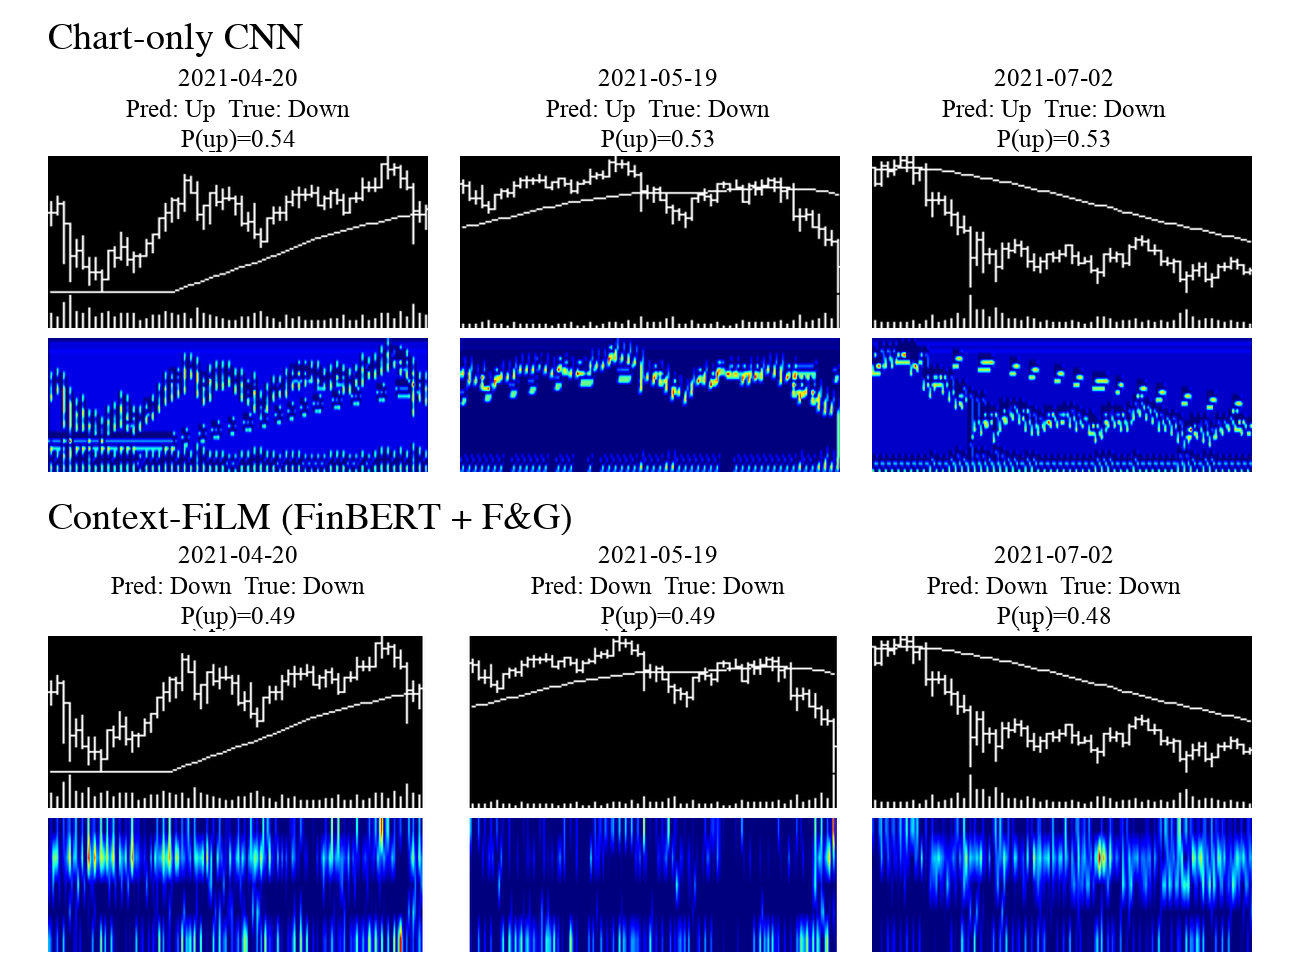
\includegraphics[width=0.96\textwidth]{gradcam_finbert_fg_corrections_chronological.png}
\caption{Correction examples with Grad-CAM and context-FiLM modulation}
\end{figure}

The limitation is important. Gamma and beta are model-internal modulation values, not event labels. A channel with positive $\Delta\gamma$ cannot be translated directly into ``fear'', ``volume'', or ``bad news''. The interpretation is therefore limited to the connection among context regime, probability transition, bounded modulation strength, and Grad-CAM saliency. This is diagnostic interpretability rather than a causal market explanation.

\clearpage

\subsection{Robustness checks}

Several robustness checks are included to clarify what kind of context is useful. Technical context is the main redundancy check: it tests whether variables derived from the same OHLCV history add information after the chart image has already been processed by the CNN. The result is close to zero, which supports the interpretation that the visual representation already captures much of this information. Generic news embeddings serve a similar role for text: they test whether semantic headline vectors are sufficient without financial sentiment alignment. Their limited effect motivates the move toward FinBERT sentiment and F\&G.

Another robustness check is the comparison between same-image and cross-image improvements. The strongest chart-only baseline uses \code{ohlc\_ma\_vb}. The derivative/leverage context improves \code{ohlc\_vb}, but it does not exceed \code{ohlc\_ma\_vb}. This does not invalidate the result; it defines its role. It is a same-image context effect and an interpretability case, while \code{ohlc\_ma\_vb} remains the strongest visual baseline.

\subsection{Why not use a fully trainable context model as the final model?}

A fully trainable context model has more capacity, and it was tested before the final protocol was chosen. The early context experiments used joint training with concatenation, gating, and FiLM-style context branches. These models allowed the visual CNN, the context branch, and the classifier to change together, but they did not provide a stable improvement over the chart-only baseline. Later ablations also tested stronger modulation and partial unfreezing. The useful lesson from these checks is that additional modulation freedom changes calibration more readily than it improves hard decisions. For this reason, the final protocol keeps the visual model fixed and uses bounded context modulation as a diagnostic correction mechanism.

The final protocol therefore freezes the trained CNN and classifier and trains only the context encoder and FiLM heads. The goal is not to maximize capacity, but to isolate the marginal role of context. If the output probability changes under this protocol, the change is attributable to the bounded context-modulation path rather than to a newly learned visual filter. This makes the interpretation cleaner, especially when the measured effects are small.

\subsection{Practical interpretation of small effects}

The numerical gains in this thesis are small. In financial machine learning, this is not surprising. Directional prediction is noisy, and a strong baseline already captures much of the available signal. The practical question is whether the context effect is consistent, explainable, and aligned with the intended economic mechanism.

The best results satisfy this weaker but more realistic criterion. F\&G and FinBERT+F\&G reduce the probability of some bullish predictions and correct a small number of false-Up samples. Derivatives context similarly reduces weak bullish predictions in leverage-related conditions. These effects are not large enough to claim a dominant forecasting system, but they are strong enough to support the thesis claim that external context can act as bounded calibration.

\subsection{Scope of the evidence}

The results should be interpreted within the scope of the available BTC sample. The test set is much smaller than the equity universe used in the original chart-image setting, so small accuracy improvements should not be treated as universal market laws. They are evidence of a measurable context effect under the specified data split and horizon.

Context timing is handled conservatively. Rolling features use past values, publication-sensitive variables are lagged, and normalization statistics are fitted on the training split. This does not remove every practical complication of real-time deployment, but it is sufficient for an offline thesis experiment and avoids the main lookahead problem. One remaining limitation is that training and validation are randomly mixed inside the pre-2021 pool. With 60-day images and 20-day forward labels, nearby samples overlap, so validation performance may be optimistic for checkpoint selection. The final evaluation is therefore framed around the held-out post-2021 test set, not around validation accuracy.

Because many context families were explored, the thesis does not rely on a single best row. The main conclusions are based on repeated patterns: chart-derived context is mostly redundant, sentiment-aligned context is more useful than generic text embeddings, and derivatives/leverage context can improve the same volume-aware image baseline in selected regimes. Grad-CAM and gamma/beta summaries are therefore used as diagnostic evidence, not as causal proof.

\subsection{Implications for model design}

The results suggest a practical design rule. If a feature can be drawn into the chart image, it may be better to encode it visually. If a feature is external to the chart, such as sentiment or leverage, it can be tested as bounded context. This distinction helps avoid adding redundant indicators and focuses future work on genuinely complementary signals.

\clearpage

\section{Conclusion}

\subsection{Summary of contributions}

This thesis studied context-conditioned FiLM for Bitcoin market-regime classification from chart images. The work first adapted a Re-image-style visual pipeline to BTC data and used the chart-only experiments to select a strong visual reference model. It then tested whether external context can improve or explain this visual predictor through a controlled FiLM interface.

The strongest chart-only baseline is \code{ohlc\_ma\_vb}. Most chart-derived technical context features do not improve it, supporting the conclusion that the image already contains much of the technical information available in OHLCV history. External context is more informative, but its effect is modest. F\&G sentiment and FinBERT+F\&G news sentiment provide small improvements on the strongest visual baseline, while funding plus CFTC open-interest context improves a same-image \code{ohlc\_vb} baseline and provides a useful leverage-context case study. The main methodological contribution is therefore not a large forecasting improvement, but a baseline-preserving protocol for testing whether market context acts as a bounded calibration signal.

\subsection{Answers to research questions}

\textbf{RQ1.} External market and news context can improve over a strong BTC chart-image baseline, but only in a limited and context-dependent way. Chart-derived variables such as Bollinger features, MFI, and volatility are mostly redundant with the visual representation. In contrast, sentiment-oriented and leverage-oriented variables are more complementary. The best news-context result is FinBERT+F\&G, and the clearest structured-context case is funding plus CFTC open interest on the \code{ohlc\_vb} image baseline.

\textbf{RQ2.} The baseline-preserving FiLM design is more interpretable than unrestricted fusion because it keeps the visual CNN and classifier fixed. Earlier joint-training variants with concatenation, gating, and unrestricted FiLM were more flexible, but they did not provide a stable improvement and made it harder to separate context usefulness from changes in visual filters. The final frozen bounded FiLM protocol gives a cleaner answer: context is allowed to make small channel-wise corrections, and those corrections can be inspected through gamma/beta summaries.

\textbf{RQ3.} Context helps mainly in selected regimes rather than uniformly across the whole test set. The strongest effects appear near uncertain chart-only predictions, active sentiment or news regimes, and some leverage-pressure conditions. Grad-CAM examples, correction/regression tables, and gamma/beta summaries suggest that bounded FiLM usually behaves as conservative probability calibration: in these context regimes it slightly adjusts the visual model's confidence and occasionally changes borderline decisions. This should be read as diagnostic interpretability, not as a causal explanation that news or F\&G directly caused the subsequent return.

\subsection{Future work}

Future work can extend this study in several directions. First, the sample size can be increased by using a longer BTC history or by evaluating the same protocol across multiple liquid crypto assets. A larger cross-asset sample would make it possible to test whether the small context effects observed here are specific to Bitcoin or represent a broader property of cryptocurrency chart-image prediction. Second, news context can be made more event-aware. Instead of using only generic embeddings or sentiment probabilities, headlines can be classified by event type, expected direction, impact horizon, and confidence before being passed to the context MLP. Third, the context horizon can be aligned more carefully with the return horizon, since short-lived news, slower sentiment regimes, and derivatives positioning may operate on different time scales. Finally, future models can test stronger but still controlled FiLM mechanisms, including uncertainty-gated modulation and partially unfrozen classifiers, while preserving the central requirement that the context effect remains measurable against a fixed visual baseline.

\clearpage

\section*{References}
\addcontentsline{toc}{section}{References}

\begingroup
\small
\sloppy
\begin{enumerate}[label={[\arabic*]},leftmargin=1.1cm,itemsep=0.35em]
\item Jiang J., Kelly B. T., Xiu D. (Re-)Imag(in)ing Price Trends // Journal of Finance. --- 2023. --- Vol. 78, No. 6. --- P. 3193--3249. --- DOI: 10.1111/jofi.13268.

\item Perez E., Strub F., de Vries H., Dumoulin V., Courville A. FiLM: Visual Reasoning with a General Conditioning Layer // Proceedings of the Thirty-Second AAAI Conference on Artificial Intelligence (AAAI-18). --- 2018. --- URL: \url{https://arxiv.org/abs/1709.07871} (accessed: 10.06.2026).

\item Selvaraju R. R., Cogswell M., Das A., Vedantam R., Parikh D., Batra D. Grad-CAM: Visual Explanations from Deep Networks via Gradient-Based Localization // Proceedings of the IEEE International Conference on Computer Vision (ICCV). --- 2017. --- P. 618--626. --- DOI: 10.1109/ICCV.2017.74.

\item Chen Y., Kelly B. T., Xiu D. Expected Returns and Large Language Models. --- SSRN working paper. --- 2022. --- URL: \url{https://ssrn.com/abstract=4416687} (accessed: 10.06.2026).

\item Lopez-Lira A., Tang Y. Can ChatGPT Forecast Stock Price Movements? Return Predictability and Large Language Models. --- 2023. --- arXiv:2304.07619. --- URL: \url{https://arxiv.org/abs/2304.07619} (accessed: 10.06.2026).

\item OpenAI. Vector embeddings and text-embedding-3-small documentation [Electronic resource]. --- URL: \url{https://developers.openai.com/api/docs/guides/embeddings} (accessed: 10.06.2026).

\item Devlin J., Chang M.-W., Lee K., Toutanova K. BERT: Pre-training of Deep Bidirectional Transformers for Language Understanding // Proceedings of NAACL-HLT 2019. --- 2019. --- P. 4171--4186. --- DOI: 10.18653/v1/N19-1423.

\item Araci D. FinBERT: Financial Sentiment Analysis with Pre-trained Language Models. --- 2019. --- arXiv:1908.10063. --- URL: \url{https://arxiv.org/abs/1908.10063} (accessed: 10.06.2026).

\item ProsusAI. FinBERT model card [Electronic resource]. --- Hugging Face. --- URL: \url{https://huggingface.co/ProsusAI/finbert} (accessed: 10.06.2026).

\item Alternative.me. Crypto Fear and Greed Index [Electronic resource]. --- URL: \url{https://alternative.me/crypto/fear-and-greed-index/} (accessed: 10.06.2026).

\item Anugrah N. BITCOIN Historical Datasets 2018--2026 Binance API [Dataset]. --- Kaggle. --- URL: \url{https://www.kaggle.com/datasets/novandraanugrah/bitcoin-historical-datasets-2018-2024} (accessed: 10.06.2026).

\item edaschau. bitcoin\_news [Dataset]. --- Hugging Face Datasets. --- URL: \url{https://huggingface.co/datasets/edaschau/bitcoin_news} (accessed: 10.06.2026).

\item BitMEX. Get Funding History: REST API documentation [Electronic resource]. --- URL: \url{https://docs.bitmex.com/api-explorer/get-funding} (accessed: 10.06.2026).

\item Commodity Futures Trading Commission. Commitments of Traders: CME Futures Only [Electronic resource]. --- URL: \url{https://www.cftc.gov/dea/futures/deacmesf.htm} (accessed: 10.06.2026).

\item Office of Financial Research. OFR Financial Stress Index [Electronic resource]. --- URL: \url{https://www.financialresearch.gov/financial-stress-index/} (accessed: 10.06.2026).

\item Federal Reserve Bank of St. Louis. FRED Economic Data [Electronic resource]. --- URL: \url{https://fred.stlouisfed.org/} (accessed: 10.06.2026).

\item Yahoo Finance. Market Data [Electronic resource]. --- URL: \url{https://finance.yahoo.com/} (accessed: 10.06.2026).

\item lich99. Stock\_CNN: PyTorch Implementation of (Re-)Imag(in)ing Price Trends [Source code]. --- GitHub. --- URL: \url{https://github.com/lich99/Stock_CNN} (accessed: 10.06.2026).

\item Perez E. FiLM: Visual Reasoning with a General Conditioning Layer [Source code]. --- GitHub. --- URL: \url{https://github.com/ethanjperez/film} (accessed: 10.06.2026).
\end{enumerate}
\endgroup

\clearpage

\section*{Appendix A. Reproducibility Artifacts}
\addcontentsline{toc}{section}{Appendix A. Reproducibility Artifacts}

The final repository should connect each numerical claim in the thesis to a summarized artifact. The working materials include visual baseline tables, image-specification comparisons, structured-context experiments, news-context experiments, correction/regression tables, and targeted Grad-CAM/modulation exports. These files are not copied into the thesis text directly; they are used to construct final tables and figures. Appendix B summarizes the experimental logic with compact code-style protocol blocks rather than full implementation code.

\begin{center}
\begin{longtable}{p{0.30\textwidth}p{0.52\textwidth}}
\toprule
\textbf{Artifact type} & \textbf{Role in the thesis}\\
\midrule
Visual baseline summary & Supports the choice of the $I60/R20$ chart-only baseline\\
Image-specification comparison & Shows the contribution of moving-average and volume information inside chart images\\
Context-source comparison & Separates redundant chart-derived context from external market context\\
News/sentiment report & Supports the FinBERT + F\&G calibration result\\
Correction/regression tables & Quantify where context corrects or harms chart-only predictions\\
Grad-CAM and modulation exports & Provide qualitative explanation for selected samples\\
\bottomrule
\end{longtable}
\end{center}

\clearpage

\section*{Appendix B. Experimental Protocols}
\addcontentsline{toc}{section}{Appendix B. Experimental Protocols}

This appendix summarizes the implementation logic in compact code-style form. It is not a replacement for the repository code, the original public chart-CNN implementation [18], or the public FiLM implementation [19]. The goal is to show the experimental flow without including file paths, API keys, or full Kaggle notebooks.

\subsection*{Protocol B1. Chart-only baseline screening}

\begin{lstlisting}[style=protocol]
INPUT:
    btc_ohlcv
    image_windows   = [5, 20, 60]
    return_horizons = [5, 20, 60]
    image_specs     = ["ohlc", "ohlc_ma", "ohlc_vb", "ohlc_ma_vb"]
    seeds_screen    = [42]
    seeds_confirm   = [42, 43, 44, 45, 46]

FOR each image_window IN image_windows:
    FOR each return_horizon IN return_horizons:
        labels = sign(future_return(return_horizon))

        FOR each image_spec IN image_specs:
            images = render_chart_images(
                btc_ohlcv,
                image_window=image_window,
                image_spec=image_spec
            )

            result_seed1 = train_chart_cnn(
                images,
                labels,
                split=(
                    "chronological post-2021 test; "
                    "random train/validation inside pre-2021 pool"
                ),
                seed=42
            )

            IF result_seed1.accuracy <= majority_class_accuracy:
                reject_candidate()
            ELSE IF result_seed1.roc_auc is weak:
                reject_candidate()
            ELSE:
                add_to_five_seed_candidates()

FOR each candidate IN five_seed_candidates:
    run_five_seed_training(candidate, seeds_confirm)
    summarize_mean_std(candidate)

SELECT visual_baseline by:
    stable five-seed accuracy,
    ROC-AUC,
    and consistency across seeds.

OUTPUT:
    selected_visual_baseline = I60/R20/ohlc_ma_vb
\end{lstlisting}

\subsection*{Protocol B2. Frozen bounded FiLM training}

\begin{lstlisting}[style=protocol]
INPUT:
    selected_visual_checkpoint
    context_features_by_date
    train_validation_test_split
    modulation_scale = 0.02

model = load_chart_only_cnn(selected_visual_checkpoint)
freeze(model.cnn_backbone)
freeze(model.classifier)

context_mlp = initialize_context_mlp()

FOR each batch:
    image_batch, context_batch, label_batch = batch

    visual_feature = model.cnn_backbone(image_batch)

    raw_gamma, raw_beta = context_mlp(context_batch)

    gamma = 1.0 + modulation_scale * tanh(raw_gamma)
    beta  =       modulation_scale * tanh(raw_beta)

    modulated_feature = gamma * visual_feature + beta
    probability_up = model.classifier(modulated_feature)

    loss = binary_cross_entropy(probability_up, label_batch)
    update(context_mlp only)

SELECT checkpoint by validation performance.

OUTPUT:
    context_film_model
    test_predictions
    gamma_beta_summaries
\end{lstlisting}

\subsection*{Protocol B3. Context construction and no-lookahead alignment}

\begin{lstlisting}[style=protocol]
INPUT SOURCES:
    Fear and Greed index
    Bitcoin news headlines
    FinBERT sentiment probabilities
    funding rates
    CFTC open interest
    macro stress proxies
    chart-derived technical controls

FOR each source:
    convert raw observations into daily records
    apply source-specific publication lag if needed
    build trailing-window features over [7, 20, 60] days

FOR news headlines:
    group headlines by date
    build one or more text representations:
        TF-IDF/SVD
        OpenAI embedding aggregates
        FinBERT sentiment aggregates

FOR slow public reports:
    use value only after release date
    forward-fill until the next observable value

FIT on training split only:
    missing-value rule
    clipping thresholds
    standardization statistics
    dimensionality reduction, if used

APPLY fitted transforms to validation and test splits.

MERGE:
    chart sample at date t
    with context values observable at or before date t

ASSERT:
    no context value uses future information
    no validation/test statistic is used during fitting

OUTPUT:
    date_aligned_context_matrix
\end{lstlisting}

\end{document}
